% The sponge construction [FIPS 202, §4, Figure 7]: the padded message P_0 ... P_{n-1} is
% XORed into the first r bits of the state, with f applied after each block (absorbing);
% then r bits are output at a time, with f applied between them (squeezing).
% Original drawing for the Hash library.
\documentclass[tikz,border=6pt]{standalone}
\usepackage[T1]{fontenc}
\usepackage{lmodern}
% Shared style for the Hash diagrams.
% Palette: Okabe–Ito (colour-blind safe). Every diagram is drawn on an opaque white card so it
% stays legible on dark page themes.
\usetikzlibrary{arrows.meta,positioning,calc,fit,backgrounds}
\definecolor{hsblue}{HTML}{0072B2}
\definecolor{hsorange}{HTML}{E69F00}
\definecolor{hsgreen}{HTML}{009E73}
\definecolor{hsvermilion}{HTML}{D55E00}
\definecolor{hspurple}{HTML}{CC79A7}
\definecolor{hsink}{HTML}{1F2933}
\tikzset{
  >={Stealth[length=2.2mm]},
  every node/.style={font=\sffamily\small, text=hsink},
  wire/.style={draw=hsink, line width=0.6pt, ->},
  reg/.style={draw=hsink, line width=0.6pt, fill=hsblue!12, minimum width=9mm, minimum height=7mm},
  fn/.style={draw=hsink, line width=0.6pt, fill=hsorange!25, rounded corners=2pt, minimum width=10mm, minimum height=6mm},
  input/.style={draw=hsink, line width=0.6pt, fill=hsgreen!20, minimum width=9mm, minimum height=6mm},
  add/.style={circle, draw=hsink, line width=0.6pt, fill=white, inner sep=0pt, minimum size=5mm, font=\sffamily\bfseries},
  card/.style={fill=white, rounded corners=4pt},
}

\begin{document}
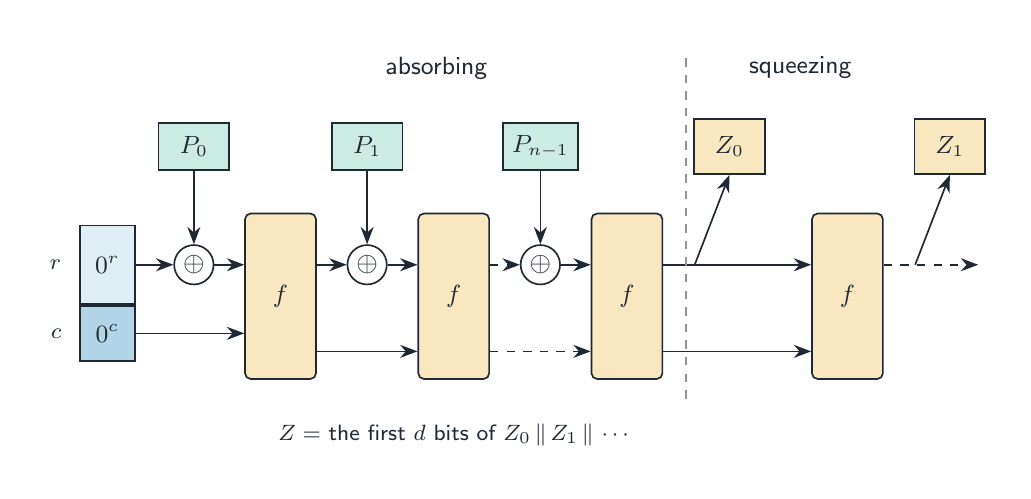
\begin{tikzpicture}[st/.style={draw=hsink, line width=0.6pt, minimum width=7mm}]
  \def\dx{2.2}
  % The initial state: r bits and c bits.
  \node[st, fill=hsblue!12, minimum height=10mm] (r0) at (0,0.5) {$0^r$};
  \node[st, fill=hsblue!30, minimum height=7mm, anchor=north] (c0) at (r0.south) {$0^c$};
  \foreach \i/\lbl in {1/P_0,2/P_1,3/P_{n-1}} {
    \node[add] (x\i) at (\i*\dx-1.1, 0.5) {$\oplus$};
    \node[input] (P\i) at (\i*\dx-1.1, 2.0) {$\lbl$};
    \draw[wire] (P\i) -- (x\i);
    \node[fn, minimum height=21mm, minimum width=9mm] (f\i) at (\i*\dx, 0.1) {$f$};
  }
  \draw[wire] (r0.east) -- (x1.west);
  \draw[wire] (x1.east) -- (x1.east -| f1.west);
  \draw[wire] (c0.east) -- (c0.east -| f1.west);
  \draw[wire] ($(f1.east)+(0,0.4)$) -- (x2.west);
  \draw[wire] (x2.east) -- (x2.east -| f2.west);
  \draw[wire] ($(f1.east)+(0,-0.7)$) -- ($(f2.west)+(0,-0.7)$);
  \draw[wire, dashed] ($(f2.east)+(0,0.4)$) -- (x3.west);
  \draw[wire] (x3.east) -- (x3.east -| f3.west);
  \draw[wire, dashed] ($(f2.east)+(0,-0.7)$) -- ($(f3.west)+(0,-0.7)$);
  % Squeezing.
  \node[fn, minimum height=21mm, minimum width=9mm] (g1) at (4*\dx+0.6, 0.1) {$f$};
  \draw[wire] ($(f3.east)+(0,0.4)$) -- ($(g1.west)+(0,0.4)$);
  \draw[wire] ($(f3.east)+(0,-0.7)$) -- ($(g1.west)+(0,-0.7)$);
  \node[reg, fill=hsorange!25] (Z0) at (3*\dx+1.3, 2.0) {$Z_0$};
  \node[reg, fill=hsorange!25] (Z1) at (4*\dx+1.9, 2.0) {$Z_1$};
  \draw[wire] ($(f3.east)+(0.4,0.4)$) -- (Z0.south);
  \draw[wire] ($(g1.east)+(0.4,0.4)$) -- (Z1.south);
  \draw[wire, dashed] ($(g1.east)+(0,0.4)$) -- ++(1.2,0);
  \node[font=\sffamily\small] at (1.9*\dx, 3.0) {absorbing};
  \node[font=\sffamily\small] at (4.0*\dx, 3.0) {squeezing};
  \draw[hsink!50, dashed] (3*\dx+0.75, -1.2) -- (3*\dx+0.75, 3.2);
  \node[anchor=east, font=\footnotesize] at ($(r0.west)+(-0.1,0)$) {$r$};
  \node[anchor=east, font=\footnotesize] at ($(c0.west)+(-0.1,0)$) {$c$};
  \node[anchor=north, font=\sffamily\footnotesize] at (2*\dx, -1.4)
    {$Z = $ the first $d$ bits of $Z_0 \,\|\, Z_1 \,\|\, \cdots$};
  \begin{scope}[on background layer]
    \coordinate (e1) at (3*\dx+3,-1.9);
    \coordinate (e2) at (-0.8,3.3);
    \node[card, fit=(r0)(c0)(P1)(Z1)(g1)(e1)(e2), inner sep=6pt] {};
  \end{scope}
\end{tikzpicture}
\end{document}
